\documentclass[11pt,twoside, reqno, align]{amsart}
\usepackage{cancel}
\usepackage{graphicx}
\graphicspath{ {./images/} }
% Macros for Fitch-style natural deduction. 
% Author: Peter Selinger, University of Ottawa
% Created: Jan 14, 2002
% Modified: Feb 8, 2005
% Version: 0.5
% Copyright: (C) 2002-2005 Peter Selinger
% Filename: fitch.sty
% Documentation: fitchdoc.tex
% URL: http://quasar.mathstat.uottawa.ca/~selinger/fitch/

% License:
%
% This program is free software; you can redistribute it and/or modify
% it under the terms of the GNU General Public License as published by
% the Free Software Foundation; either version 2, or (at your option)
% any later version.
%
% This program is distributed in the hope that it will be useful, but
% WITHOUT ANY WARRANTY; without even the implied warranty of
% MERCHANTABILITY or FITNESS FOR A PARTICULAR PURPOSE. See the GNU
% General Public License for more details.
%
% You should have received a copy of the GNU General Public License
% along with this program; if not, write to the Free Software Foundation, 
% Inc., 59 Temple Place, Suite 330, Boston, MA 02111-1307, USA.

% USAGE EXAMPLE:
% 
% The following is a simple example illustrating the usage of this
% package.  For detailed instructions and additional functionality, see
% the user guide, which can be found in the file fitchdoc.tex.
% 
% \[
% \begin{nd}
%   \hypo{1}  {P\vee Q}   
%   \hypo{2}  {\neg Q}                         
%   \open                              
%   \hypo{3a} {P}
%   \have{3b} {P}        \r{3a}
%   \close                   
%   \open
%   \hypo{4a} {Q}
%   \have{4b} {\neg Q}   \r{2}
%   \have{4c} {\bot}     \ne{4a,4b}
%   \have{4d} {P}        \be{4c}
%   \close                             
%   \have{5}  {P}        \oe{1,3a-3b,4a-4d}                 
% \end{nd}
% \]

{\chardef\x=\catcode`\*
\catcode`\*=11
\global\let\nd*astcode\x}
\catcode`\*=11

% References

\newcount\nd*ctr
\def\nd*render{\expandafter\ifx\expandafter\nd*x\nd*base\nd*x\the\nd*ctr\else\nd*base\ifnum\nd*ctr<0\the\nd*ctr\else\ifnum\nd*ctr>0+\the\nd*ctr\fi\fi\fi}
\expandafter\def\csname nd*-\endcsname{}

\def\nd*num#1{\nd*numo{\nd*render}{#1}\global\advance\nd*ctr1}
\def\nd*numopt#1#2{\nd*numo{$#1$}{#2}}
\def\nd*numo#1#2{\edef\x{#1}\mbox{$\x$}\expandafter\global\expandafter\let\csname nd*-#2\endcsname\x}
\def\nd*ref#1{\expandafter\let\expandafter\x\csname nd*-#1\endcsname\ifx\x\relax%
  \errmessage{Undefined natdeduction reference: #1}\else\mbox{$\x$}\fi}
\def\nd*noop{}
\def\nd*set#1#2{\ifx\relax#1\nd*noop\else\global\def\nd*base{#1}\fi\ifx\relax#2\relax\else\global\nd*ctr=#2\fi}
\def\nd*reset{\nd*set{}{1}}
\def\nd*refa#1{\nd*ref{#1}}
\def\nd*aux#1#2{\ifx#2-\nd*refa{#1}--\def\nd*c{\nd*aux{}}%
  \else\ifx#2,\nd*refa{#1}, \def\nd*c{\nd*aux{}}%
  \else\ifx#2;\nd*refa{#1}; \def\nd*c{\nd*aux{}}%
  \else\ifx#2.\nd*refa{#1}. \def\nd*c{\nd*aux{}}%
  \else\ifx#2)\nd*refa{#1})\def\nd*c{\nd*aux{}}%
  \else\ifx#2(\nd*refa{#1}(\def\nd*c{\nd*aux{}}%
  \else\ifx#2\nd*end\nd*refa{#1}\def\nd*c{}%
  \else\def\nd*c{\nd*aux{#1#2}}%
  \fi\fi\fi\fi\fi\fi\fi\nd*c}
\def\ndref#1{\nd*aux{}#1\nd*end}

% Layer A

% define various dimensions (explained in fitchdoc.tex):
\newlength{\nd*dim} 
\newdimen\nd*depthdim
\newdimen\nd*hsep
\newdimen\ndindent
\ndindent=1em
% user command to redefine dimensions
\def\nddim#1#2#3#4#5#6#7#8{\nd*depthdim=#3\relax\nd*hsep=#6\relax%
\def\nd*height{#1}\def\nd*thickness{#8}\def\nd*initheight{#2}%
\def\nd*indent{#5}\def\nd*labelsep{#4}\def\nd*justsep{#7}}
% set initial dimensions
\nddim{4.5ex}{3.5ex}{1.5ex}{1em}{1.6em}{.5em}{2.5em}{.2mm}

\def\nd*v{\rule[-\nd*depthdim]{\nd*thickness}{\nd*height}}
\def\nd*t{\rule[-\nd*depthdim]{0mm}{\nd*height}\rule[-\nd*depthdim]{\nd*thickness}{\nd*initheight}}
\def\nd*i{\hspace{\nd*indent}} 
\def\nd*s{\hspace{\nd*hsep}}
\def\nd*g#1{\nd*f{\makebox[\nd*indent][c]{$#1$}}}
\def\nd*f#1{\raisebox{0pt}[0pt][0pt]{$#1$}}
\def\nd*u#1{\makebox[0pt][l]{\settowidth{\nd*dim}{\nd*f{#1}}%
    \addtolength{\nd*dim}{2\nd*hsep}\hspace{-\nd*hsep}\rule[-\nd*depthdim]{\nd*dim}{\nd*thickness}}\nd*f{#1}}

% Lists

\def\nd*push#1#2{\expandafter\gdef\expandafter#1\expandafter%
  {\expandafter\nd*cons\expandafter{#1}{#2}}}
\def\nd*pop#1{{\def\nd*nil{\gdef#1{\nd*nil}}\def\nd*cons##1##2%
    {\gdef#1{##1}}#1}}
\def\nd*iter#1#2{{\def\nd*nil{}\def\nd*cons##1##2{##1#2{##2}}#1}}
\def\nd*modify#1#2#3{{\def\nd*nil{\gdef#1{\nd*nil}}\def\nd*cons##1##2%
    {\advance#2-1 ##1\advance#2 1 \ifnum#2=1\nd*push#1{#3}\else%
      \nd*push#1{##2}\fi}#1}}

\def\nd*cont#1{{\def\nd*t{\nd*v}\def\nd*v{\nd*v}\def\nd*g##1{\nd*i}%
    \def\nd*i{\nd*i}\def\nd*nil{\gdef#1{\nd*nil}}\def\nd*cons##1##2%
    {##1\expandafter\nd*push\expandafter#1\expandafter{##2}}#1}}

% Layer B

\newcount\nd*n
\def\nd*beginb{\begingroup\nd*reset\gdef\nd*stack{\nd*nil}\nd*push\nd*stack{\nd*t}%
  \begin{array}{l@{\hspace{\nd*labelsep}}l@{\hspace{\nd*justsep}}l}}
\def\nd*resumeb{\begingroup\begin{array}{l@{\hspace{\nd*labelsep}}l@{\hspace{\nd*justsep}}l}}
\def\nd*endb{\end{array}\endgroup}
\def\nd*hypob#1#2{\nd*f{\nd*num{#1}}&\nd*iter\nd*stack\relax\nd*cont\nd*stack\nd*s\nd*u{#2}&}
\def\nd*haveb#1#2{\nd*f{\nd*num{#1}}&\nd*iter\nd*stack\relax\nd*cont\nd*stack\nd*s\nd*f{#2}&}
\def\nd*havecontb#1#2{&\nd*iter\nd*stack\relax\nd*cont\nd*stack\nd*s\nd*f{\hspace{\ndindent}#2}&}
\def\nd*hypocontb#1#2{&\nd*iter\nd*stack\relax\nd*cont\nd*stack\nd*s\nd*u{\hspace{\ndindent}#2}&}

\def\nd*openb{\nd*push\nd*stack{\nd*i}\nd*push\nd*stack{\nd*t}}
\def\nd*closeb{\nd*pop\nd*stack\nd*pop\nd*stack}
\def\nd*guardb#1#2{\nd*n=#1\multiply\nd*n by 2 \nd*modify\nd*stack\nd*n{\nd*g{#2}}}

% Layer C

\def\nd*clr{\gdef\nd*cmd{}\gdef\nd*typ{\relax}}
\def\nd*sto#1#2#3{\gdef\nd*typ{#1}\gdef\nd*byt{}%
  \gdef\nd*cmd{\nd*typ{#2}{#3}\nd*byt\\}}
\def\nd*chtyp{\expandafter\ifx\nd*typ\nd*hypocontb\def\nd*typ{\nd*havecontb}\else\def\nd*typ{\nd*haveb}\fi}
\def\nd*hypoc#1#2{\nd*chtyp\nd*cmd\nd*sto{\nd*hypob}{#1}{#2}}
\def\nd*havec#1#2{\nd*cmd\nd*sto{\nd*haveb}{#1}{#2}}
\def\nd*hypocontc#1{\nd*chtyp\nd*cmd\nd*sto{\nd*hypocontb}{}{#1}}
\def\nd*havecontc#1{\nd*cmd\nd*sto{\nd*havecontb}{}{#1}}
\def\nd*by#1#2{\ifx\nd*x#2\nd*x\gdef\nd*byt{\mbox{#1}}\else\gdef\nd*byt{\mbox{#1, \ndref{#2}}}\fi}

% multi-line macros
\def\nd*mhypoc#1#2{\nd*mhypocA{#1}#2\\\nd*stop\\}
\def\nd*mhypocA#1#2\\{\nd*hypoc{#1}{#2}\nd*mhypocB}
\def\nd*mhypocB#1\\{\ifx\nd*stop#1\else\nd*hypocontc{#1}\expandafter\nd*mhypocB\fi}
\def\nd*mhavec#1#2{\nd*mhavecA{#1}#2\\\nd*stop\\}
\def\nd*mhavecA#1#2\\{\nd*havec{#1}{#2}\nd*mhavecB}
\def\nd*mhavecB#1\\{\ifx\nd*stop#1\else\nd*havecontc{#1}\expandafter\nd*mhavecB\fi}
\def\nd*mhypocontc#1{\nd*mhypocB#1\\\nd*stop\\}
\def\nd*mhavecontc#1{\nd*mhavecB#1\\\nd*stop\\}

\def\nd*beginc{\nd*beginb\nd*clr}
\def\nd*resumec{\nd*resumeb\nd*clr}
\def\nd*endc{\nd*cmd\nd*endb}
\def\nd*openc{\nd*cmd\nd*clr\nd*openb}
\def\nd*closec{\nd*cmd\nd*clr\nd*closeb}
\let\nd*guardc\nd*guardb

% Layer D

% macros with optional arguments spelled-out
\def\nd*hypod[#1][#2]#3[#4]#5{\ifx\relax#4\relax\else\nd*guardb{1}{#4}\fi\nd*mhypoc{#3}{#5}\nd*set{#1}{#2}}
\def\nd*haved[#1][#2]#3[#4]#5{\ifx\relax#4\relax\else\nd*guardb{1}{#4}\fi\nd*mhavec{#3}{#5}\nd*set{#1}{#2}}
\def\nd*havecont#1{\nd*mhavecontc{#1}}
\def\nd*hypocont#1{\nd*mhypocontc{#1}}
\def\nd*base{undefined}
\def\nd*opend[#1]#2{\nd*cmd\nd*clr\nd*openb\nd*guard{#1}#2}
\def\nd*close{\nd*cmd\nd*clr\nd*closeb}
\def\nd*guardd[#1]#2{\nd*guardb{#1}{#2}}

% Handling of optional arguments.

\def\nd*optarg#1#2#3{\ifx[#3\def\nd*c{#2#3}\else\def\nd*c{#2[#1]{#3}}\fi\nd*c}
\def\nd*optargg#1#2#3{\ifx[#3\def\nd*c{#1#3}\else\def\nd*c{#2{#3}}\fi\nd*c}

\def\nd*five#1{\nd*optargg{\nd*four{#1}}{\nd*two{#1}}}
\def\nd*four#1[#2]{\nd*optarg{0}{\nd*three{#1}[#2]}}
\def\nd*three#1[#2][#3]#4{\nd*optarg{}{#1[#2][#3]{#4}}}
\def\nd*two#1{\nd*three{#1}[\relax][]}

\def\nd*have{\nd*five{\nd*haved}}
\def\nd*hypo{\nd*five{\nd*hypod}}
\def\nd*open{\nd*optarg{}{\nd*opend}}
\def\nd*guard{\nd*optarg{1}{\nd*guardd}}

\def\nd*init{%
  \let\open\nd*open%
  \let\close\nd*close%
  \let\hypo\nd*hypo%
  \let\have\nd*have%
  \let\hypocont\nd*hypocont%
  \let\havecont\nd*havecont%
  \let\by\nd*by%
  \let\guard\nd*guard%
  \def\ii{\by{$\Rightarrow$I}}%
  \def\ie{\by{$\Rightarrow$E}}%
  \def\Ai{\by{$\forall$I}}%
  \def\Ae{\by{$\forall$E}}%
  \def\Ei{\by{$\exists$I}}%
  \def\Ee{\by{$\exists$E}}%
  \def\ai{\by{$\wedge$I}}%
  \def\ae{\by{$\wedge$E}}%
  \def\ai{\by{$\wedge$I}}%
  \def\ae{\by{$\wedge$E}}%
  \def\oi{\by{$\vee$I}}%
  \def\oe{\by{$\vee$E}}%
  \def\ni{\by{$\neg$I}}%
  \def\ne{\by{$\neg$E}}%
  \def\be{\by{$\bot$E}}%
  \def\nne{\by{$\neg\neg$E}}%
  \def\r{\by{R}}%
}

\newenvironment{nd}{\begingroup\nd*init\nd*beginc}{\nd*endc\endgroup}
\newenvironment{ndresume}{\begingroup\nd*init\nd*resumec}{\nd*endc\endgroup}

\catcode`\*=\nd*astcode

% End of file fitch.sty



%%%%%%%%%%%%%%%%%%%%%%%%%%%%%%%packages%%%%%%%%%%%%%%%%%%%


%%%%%%%%%%%%%%%%%%%%%%%%%%%%%%%formatting%%%%%%%%%%%%%%%%%%

\setlength{\topmargin}{0in} 
\setlength{\oddsidemargin}{0in}   
\setlength{\evensidemargin}{0in}  
\setlength{\textheight}{8.5in}    
\setlength{\textwidth}{6.5in}  
\setlength{\headsep}{0.15in}   
\setlength{\headheight}{0in}
\parskip=4pt 

%%%%%%%%%%%%%%%%%%%%%%%%%%%%%%%formatting%%%%%%%%%%%%%%%%%%

\newtheorem{Thm}{Theorem}
\newtheorem{Def}[Thm]{Definition}
\newtheorem{Lm}[Thm]{Lemma}
\newtheorem{Prop}[Thm]{Proposition}
\newtheorem{Cor}[Thm]{Corollary}


\theoremstyle{remark}
\newtheorem{Rem}[Thm]{Remark}
\newtheorem{Exp}[Thm]{Example}
\newtheorem{Prob}{Problem}

%\numberwithin{equation}{section}



\def\R{\mathbb R}
\def\Q{\mathbb Q}
\def\N{\mathbb N}
\def\Z{\mathbb Z}
\def\P{\mathbb P}


%%%%%%%%%%%%%%%%logical connectors%%%%%%%%%%%%%%%%%%%%%%%%%%%%%%%%%%%%%

\newcommand{\OR}{\vee}
\newcommand{\AND}{\wedge}
\renewcommand{\implies}{\Rightarrow}
\newcommand{\implied}{\Leftarrow}
\renewcommand{\iff}{\Leftrightarrow}

%%%%%%%%%%%%%%%%%%%%%%%%%%%%%%%%%%%%%%%%%%%%%%%%%%%%%

\begin{document}
\title{Math 0450: Homework 3}
\date{\today}
\author{Teoh Zhixiang}

\maketitle



\begin{Prob}
Let $L=\{q\in \Q~|~q^2<2\}$. Show that  if $q>0$ and $q\in L$ then $q^\prime=2(q+1)/(q+2)\in L$ and $q<q^\prime$. Deduce that $L$ does not have a maximal element.
\end{Prob}

\begin{proof}
\begin{align*}
    (q')^2 & = \frac{(2(q+1))^2}{(q+2)^2} \\
    & = \frac{4(q^2 + 2q + 1)}{q^2 + 2q + 4} \\
    & = 4 - \frac{12}{(q+2)^2} \\
    & < 4 - \frac{12}{(0+2)^2} \\
    & = 4 - 3 \\
    & = 1 \\
    & < 2
\end{align*}
$q'= \frac{2(q+1)}{q+2} \in \Q$ if $q \in \Q$, and $(q')^2 < 2$ if $q \in L$ as shown above, so $q' \in L$.
\begin{align*}
    q' & = \frac{2q+2}{q+2} \\
    & = \frac{q(q+2)+2-q^2}{q+2} \\
    & = q + \frac{2-q^2}{q+2} \\
    & > q
\end{align*}
since $q^2 < 2 \iff 2 - q^2 > 0$ and $0 < q < \sqrt{2} \iff q+2 > 0$. So $q < q'$.

From $q'$ we can recursively, using the formula for $q'$ above, derive a $q'' \in L$ and $q'' > q'$, and likewise for $q''' > q''$, and so on. Since for every $q \in L$ we can derive a $q < q' \in L$ from $q$, this shows there is always an element $q' > q \in L$ for every $q$, and that there is no maximal element in $L$.
\end{proof}

\paragraph{}

\begin{Prob}
Let $U=\{u\in \Q~|~u^2\geq 2\}$. Show that  if $u>0$ and $u\in U$ then $u^\prime=2(u+1)/(u+2)\in U$ and $u>u^\prime$. Deduce that $U$ does not have a minimal element.
\end{Prob}

\begin{proof}
\begin{align*}
    (u')^2 & = \frac{(2(u+1))^2}{(u+2)^2} \\
    & = \frac{4(u^2 + 2u + 1)}{u^2 + 2u + 4} \\
    & = 4 - \frac{12}{(u+2)^2} \\
    & < 4 - \frac{12}{(\sqrt{2}+2)^2} \\
    & = 4 - \frac{12}{6 + 4\sqrt{2}} \\
    & > 4 - \frac{12}{10} \\
    & = 2.8 \\
    & > 2
\end{align*}
Note at third last step $\frac{12}{6+4\sqrt{2}}$ is estimated to be $\frac{12}{10}$, and is valid because $(1 < \sqrt{2}) \iff (\frac{12}{10} > \frac{12}{6+4\sqrt{2}}) \iff (4-\frac{12}{10} < 4-\frac{12}{6+4\sqrt{2}})$, and so if $(4-\frac{12}{10} > 2) \iff (4-\frac{12}{6+4\sqrt{2}} > 2)$. $u'= \frac{2(u+1)}{u+2} \in \Q$ if $u \in \Q$, and $(u')^2 > 2$ if $u \in U$ as shown above, so $u' \in L$.
\begin{align*}
    u' & = \frac{2u+2}{u+2} \\
    & = \frac{u(u+2)+2-u^2}{u+2} \\
    & = u + \frac{2-u^2}{u+2} \\
    & < u
\end{align*}
since $u^2 > 2 \iff 2 - u^2 < 0$ and $0 < \sqrt{2} < u \iff u+2 > 0$. So $\frac{2-u^2}{u+2} < 0$, and $u > u'$. 

From $u'$ we can recursively, using the formula for $u'$ above, derive a $u'' \in U$ and $u'' < u'$, and likewise for $u''' < u''$, and so on. Since for every $u \in U$ we can derive a $u < u' \in U$ from $u$, this shows there is always an element $u' < u \in U$ for every $u$, and hence that there is no minimal element in $U$.
\end{proof}

\paragraph{}

\begin{Prob}
Let $F$ be an ordered field. Show that for any $n\geq 1$ and $a_1, a_2, \dots, a_n \in F$ we have
$$
|a_1+a_2+\cdots+a_n|\leq |a_1|+|a_2|+\cdots+|a_n|.
$$
\end{Prob}

\begin{proof}
(By induction). We first define the absolute value operation $|\cdot|$ as follows:
$$
|a| = 
\begin{cases}
    a & \text{if $a > 0$}\\
    -a & \text{if $a < 0$}\\
    0 & \text{if $a = 0$}
\end{cases}
$$
Let $P(n)$ be the statement $|a_1+a_2+\cdots+a_n|\leq |a_1|+|a_2|+\cdots+|a_n|$, for $n \geq 1$ and $a_1, a_2, \dots, a_n \in F$. We prove two base cases: $P(1)$ and $P(2)$. The first base case, $P(1)$, is trivial because $|a_1| = |a_1| \iff |a_1| \leq |a_1|$. We shall prove $P(2)$, also called the triangle inequality, i.e. $|a_1+a_2|\leq |a_1|+|a_2|$. By definition of absolute value operation, $|a_1 + a_2| \geq 0$, and $|a+b| \geq 0$. Note also
\begin{align*}
    |a|^2 & = |a|\cdot|a| \\
    \text{consider 3 cases:} \\
    a > 0: |a|^2 & = a \cdot a \\
    & = a^2 \\
    a < 0: |a|^2 & = -a \cdot -a \\
    & = a^2 \;\text{(by property of ordered field $-a \cdot -b = a \cdot b$)} \\
    a = 0: |a|^2 & = 0 \cdot 0 \\
    & =a^2 \\
    \implies |a|^2 & = a^2
\end{align*}
Therefore
\begin{align*}
    & &|a_1 + a_2| & \leq |a_1| + |a_2| \\
    & \iff & (a_1 + a_2)^2 & \leq (|a_1| + |a_2|)^2 \\
    & \iff & a_1^2 + a_2^2 + 2a_1a_2 & \leq |a_1|^2 + |a_2|^2 + 2|a_1||a_2| \\
    & & & = a_1^2 + a_2^2 + 2|a_1||a_2| \\
    & \iff & 2a_1a_2 & \leq 2|a_1||a_2| \\
    & \iff & a_1a_2 & \leq |a_1||a_2|
\end{align*}
Note $|a_1||a_2| = |a_1a_2|$: consider cases for different values of $a_1,a_2$. If $a_1, a_2 > 0$ or $a_1, a_2 < 0$, statement valid. ($a_1$ or $a_2 = 0) \implies |0| = |0|$ valid. If only either $a_1$ or $a_2 < 0$: assume $a_2 < 0$, $|a_1||a_2| = a_1(-a_2) = |-a_1a_2| > 0$, similarly for $a_1 < 0$. Therefore $a_1a_2 \leq |a_1||a_2|$ true, and $P(2)$ valid.

Next we assume $P(n)$ true for some $n \in \N$. Then
\begin{align*}
    &  & |\underbrace{a_1+a_2+\cdots+a_n}_\text{:= A} + a_{n+1}| & \leq |\underbrace{a_1+a_2+\cdots+a_n}_\text{:= A}| + |a_{n+1}| \\
    & \iff & |A + a_{n+1}| & \leq |A| + |a_{n+1}|
    % & \leq |a_1|+|a_2|+\cdots+|a_n|+|a_{n+1}| \\
    % & \iff & (a_1+a_2+\cdots+a_n+a_{n+1})^2 & \leq (|a_1|+|a_2|+\cdots+|a_n|+|a_{n+1}|)^2 \\
    % & \iff &  & \leq &
\end{align*}
By $P(2)$, the above inequality in $A$ is true. In a similar manner to the above, $P(n+1)$ can be proven in a recursive manner:
\begin{align*}
    |A| + |a_{n+1}| & = |a_1 + a_2 + \cdots + a_{n-1} + a_n| + |a_{n+1}| \\
    & \leq |\underbrace{a_1 + a_2 + \cdots + a_{n-1}}_\text{$A_2$} + a_n| + |a_{n+1}| \\
    & \leq |A_2| + |a_n| + |a_{n+1}| \\
    & \leq \ldots
\end{align*}
each time using result from $P(2)$. Therefore $P(n+1)$ true, and so by Principle of Mathematical Induction $P(n)$ true for all $n \in \N$.
\end{proof}

\paragraph{}

\begin{Prob}
Let $A$ and $B$ be two sets with $n$ and, respectively, $m$ elements. Let $f:A\to B$ a function. Show that

\begin{enumerate}
\item If $f$ injective then $n\leq m$;
\item If $f$ surjective then $n\geq m$;
\item If $f$ bijective then $n=m$.
\end{enumerate}
\end{Prob}

\begin{proof}
\begin{enumerate}
    \item (Contraposition). $f$ is said to be injective or 1-1 if for every two elements $a,b \in A$, $(f(a) = f(b)) \implies (a = b)$. Assume negation of $n \leq m$ is true, i.e. $n > m$. If $f$ is injective, then every two elements $a_1,a_2 \in A$ must have different images $b_1,b_2 \in B$ under $f$, if $f(a_1) = b_1$ and $f(a_2) = b_2$. Pigeonhole principle states that if $n > m$ containers are put into $m$ containers then at least one container must contain more than one item. So because the cardinality of the domain $|A| = n$ is greater than the cardinality of the codomain $|B| = m$, as assumed, by pigeonhole principle, there is no way to map $n > m$ elements in domain $A$ to $m$ elements in domain $B$ without at least one element in domain $B$ having more than one preimage from domain $A$. So $f$ is shown to not be injective, and by proof of contraposition we have that $f$ injective $\implies n \leq m$. 
    \\
    \item (Contraposition). $f$ is said to be surjective or onto if every element $b \in B$ has a preimage $a \in A$. Assume $n < m$. The function $f$ is defined as the relation between sets A and B that associates every element in domain $A$ to exactly one element in the codomain $B$. Hence, similarly by pigeonhole principle, we see that there is no way to map $n < m$ elements in domain $A$ to $m$ elements in domain $B$ without at least one element in domain $A$ mapping to two elements in codomain $B$, which defies the definition of a function. Thus $f$ cannot be surjective, and by proof of contraposition we have that $f$ surjective $\implies n \geq m$.
    \\
    \item Let $p \implies (r \OR s)$ be the statement in part $(1)$ and $q \implies (r \OR t)$ be the statement in part $(2)$, where $p, q, r, t, s$ represent the statements "$f$ injective", "$f$ surjective", "$n = m$", "$n < m$" and "$n > m$" respectively. Hence we can introduce a third proposition $\neg ((n < m)\AND(n > m)) \equiv \neg (s \AND t) \equiv \neg s \OR \neg t$.
    
    Now we set up a proof by cases with our three propositional statements, considering the two cases: when $\neg s$ and when $\neg t$. The following is a First Order Logic (FOL) proof in fitch format:
    
    \begin{nd}
        \hypo {1} {p \implies (r \OR t)}
        \hypo {2} {q \implies (r \OR s)}
        \hypo {3} {\neg s \OR \neg t}
        \open
            \hypo {4} {\neg t}
            \open
                \hypo {5} {p \AND q}
                \have {6} {p}                           \ae{5}
                \have {7} {r \OR t}                     \ie{1,6}
                \open    
                    \hypo {8} {r}
                    \have {9} {r}                       \r{8}
                    \close
                \open
                    \hypo {10} {t}
                    \have {11} {\neg t}                 \r{10}
                    \have {12} {\bot}                   \ne{10,11}
                    \have {13} {r}                      \be{12}
                    \close
                \have {14} {r}                          \oe{7,8-9,10-13}
                \close
            \have {15} {(p \AND q) \implies r}          \ii{5-14}
            \close
    \end{nd}
    \begin{ndresume}
        \open
            \hypo {16} {\neg s}
            \open
                \hypo {17} {p \AND q}
                \have {18} {q}                          \ae{17}
                \have {19} {r \OR s}                    \ie{2,18}
                \open    
                    \hypo {20} {r}
                    \have {21} {r}                      \r{20}
                    \close
                \open
                    \hypo {22} {s}
                    \have {23} {\neg s}                 \r{22}
                    \have {24} {\bot}                   \ne{22,23}
                    \have {25} {r}                      \be{24}
                    \close
                \have {26} {r}                          \oe{16,20-21,22-25}
                \close
            \have {27} {(p \AND q) \implies r}          \ii{17-26}
            \close
        \have {28} {(p \AND q) \implies r}              \oe{3,4-15,16-27}
        \close
    \end{ndresume}
    
    And from this we can see that statement (3): $f$ bijective $\implies n = m$ follows from statements (2) and (3).
\end{enumerate}

\end{proof}

\begin{Prob}
The set $S$ is said to be infinite if there exists a proper subset $A\subseteq S$ and an injective function $S\to A$. Show that the sets $\N$, $\Z$, and $\Q$ are infinite.
\end{Prob}

\begin{proof}
The set $A$ is defined to be a proper subset of $S$, $A \subset S$, if it satisfies $\{A \subseteq S \mid A \neq S\}$.

We first prove $\N$ is infinite. We define the set $A_1 \subset \N$ as follows:
$$
A = \{n \in \N \mid 2n\}.
$$
Note that $A_1$ is a proper subset of $S$ because every element $a \in A_1$ also belongs to $\N$, but there is at least one element in $\N$ (in fact all odd natural numbers) that is not in $A_1$. With these sets defined, we have the function $f: A_1 \to \N$, i.e. $f(2n) = n$, for all $n \in \N$. To prove $f$ is injective, we pick any two arbitrary elements $f(n_1) = f(n_2) \in \N$ and show that it must be the case that $n_1 = n_2 \in A_1$. $f(n_1) = f(n_2) \iff \frac{n_1}{\cancel{2}} = \frac{n_2}{\cancel{2}} \iff n_1 = n_2$. Therefore $f$ injective, and we have proven $\N$ infinite. 

We now prove $\Z$ is infinite. We define the set $A_2 \subset \Z$ as the set $\N$. Note that $\N$ is a proper subset of $S$ because $\Z = \N \cup \{0\} \cup (-\N)$; so every element $n \in \N$ also belongs to $\Z$, but there is at least one element in $\Z$ (in fact all non-positive integers) that is not in $\N$. Consider the function $f: \Z \to \N$ defined by:
$$
f(n) = 
\begin{cases}
    2n+1 & \text{if $n \geq 0$} \\
    -2n & \text{if $n < 0$}
\end{cases}
$$
for all $n \in \N$. Pick any two arbitrary $f(n_1) = f(n_2) \in \N$. If $f(n_1) = f(n_2)$ is odd, then $n_1 = n_2$ and is the nonnegative integer preimage that maps to the odd natural number $2n_1+1 = 2n_2+1 \iff n_1 = n_2$, else if $f(n_1) = f(n_2)$ is even then $n_1 = n_2$ and is negative. Therefore $f$ is injective, and $\Z$ is infinite.

We now prove $\Q$ is infinite. We define the set $A_3 \subset \Q$ as the set of natural numbers $\N$. Note that $\N$ is a proper subset of $\Q$ because every element in $\N$ is an element of $\Q$ (in particular all elements with denominator $1$) but there is at least one $q \in \Q$ (eg. $\frac{2}{3}$) that is not in $\N$. Consider the function $f:\Q \to \N$ defined as the mapping from elements $(a,b) = \frac{a}{b} \in \Q$ where $gcd(a,b) = 1$, for all $a,b \in \Z$. In Figure 1, imagine there are two coordinate axes pointing in the upwards and rightwards direction, corresponding to $a$ and $b$ respectively, i.e. the point $(1,0) = \frac{1}{0}$ is represented by the point $1$ as shown, even though the value might not necessarily be valid (which in this case it is not because the denominator is 0). But Figure 1 nonetheless proves that there exists an injection from $\Q$ to $\N$, because every simplest rational number $(a,b)$ can be mapped to a natural number, and each natural number has only one rational number preimage. Therefore $Q$ is infinite.
\begin{figure}
    \centering
    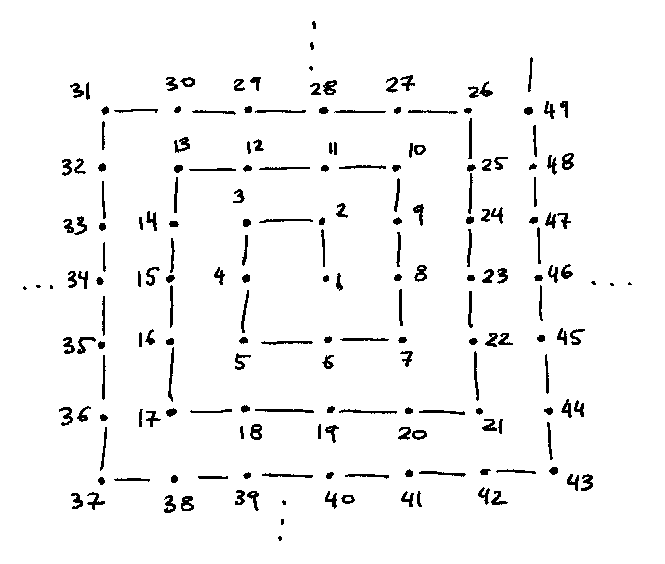
\includegraphics{QtoN.png}
    \caption{Mapping from $\Q$ to $\N$. Each point on the spiral represents an element $(a,b) \in \Q$ that is mapped to a natural number $n \in \N$.}
    \label{fig:my_label}
\end{figure}

\end{proof}

\end{document}